\chapter{Background}
Synchronous DRAM (SDRAM) was first standardised by JEDEC in 1993, and is still the foundation for modern DDR3 and DDR4 memories \cite{standard2008double}. Although the memory architecture has been improved over the years, the fundamental design has mostly been left untouched. However, there are several emerging DRAM technologies which aim at creating an entirely new and improved design: Hybrid Memory Cube (HMC), High Bandwidth Memory (HBM) and Wide-IO among others. In this chapter, we will start by describing how today's memories operate and then go on to explain how previously mentioned emerging technologies are designed and how they differ. 

%%%%%%%%%%%%%%%%%%%%%%%%%%%%%%  DDR  %%%%%%%%%%%%%%%%%%%%%%%%%%%%%%
\section{DDR SDRAM}
Being made up of just one transistor and one capacitor, the DRAM cell is small and can hold a charge for a short period of time. Because the data inside disappears after a while if left untouched, cells must be refreshed in order to not become corrupt. Every cell can store one bit and are arranged into arrays, divided into rows. The size of these rows depend on the memory technology, density and manufacturer. Each row is connected to a wordline driver, which is used to address the specific row. Arrays are ordered into \emph{banks}, which is the smallest independent unit in the memory -- in other words, requests to different banks can be serviced in parallel. When a memory address is received, it is split into row and column parts. The wordline connected to the addressed row is activated with a Row Access Strobe (RAS), the data is detected by a \emph{sense amplifier} which acts as a \emph{row buffer}. Next, data is driven into or out of the row -- depending on if the command was a read or a write -- by a Column Access Strobe (CAS). There can be subsequent accesses to the same row without the need to reread the row from the array, but if another row needs to be accessed, the sense amplifier must be emptied by a Precharge (PRE) command. Banks are grouped together into \emph{ranks}, where, for example, DDR3 uses eight banks per rank. Lastly, memory ranks are attached to both sides of a \emph{Dual Inline Memory Module} (DIMM), which in turn is then either soldered or otherwise mounted on a motherboard. 
\bigskip

Banks do not keep track of data states or timings themselves, but that is the task of the memory controller. The latter is usually situated in the Central Processing Unit (CPU), instead of on the DIMM; this saves space and hence allows for larger memories. Arrays are designed to be as simple as possible, and do not prevent data corruption in any way by themselves. All control mechanisms, e.g. timing, bus contention and row refreshing, are built in and handled by the memory controller. In order to not over-utilise buses, and enable a lower clock frequency, data is sent in bursts. For example, a sequence of read operations can be sent eight-by-eight. 

TODO: Mention that quite a large portion of the memory bus is occupied by just refresh operations (10-15-20\%) (every 60ms) and that this number increases with memory size --> more memory which need to be refreshed in the same amount of time.
TODO: Mention ECC, registered/buffered memories as well. Since other memory types, e.g., HMC has built-in ECC etc this is highly relevant in a comparison. 
\bigskip

TODO: Reference previously mentioned MLM, where DDR could either be used in conjunction with other technology than DRAM, or act as a part os the MLM... Or?
TODO: Versions of DDR - DDR3 DDR4 DDR5 LPDDR4X GDDR4 GDDR5x GDDR6. SODIMM, DIMM, Voltage levels

%%%%%%%%%%%%%%%%%%%%%%%%%%%%%%  HMC  %%%%%%%%%%%%%%%%%%%%%%%%%%%%%%
\section{Hybrid Memory Cube}
The Hybrid Memory Cube is also based on DRAM memory cells, but unlike SDRAM, it consists of multiple dies stacked on top of one another \cite{hybrid2013hybrid}. Consequently, the HMC can fit more memory onto the same packaging area, which gets even more important as HMC is designed for near-memory computation. This technology is more expensive and power hungry on its own, but its efficiency in terms of bit/s/watt is an order of magnitude higher than normal DRAM memory \cite{7477494}. Both due to its novelty and its design, HMC is also about three times more expensive than DDR memory, which means it will not be used as a replacement without doing due optimisations in both software and hardware \cite{Jayaraj:2015:PPM:2818950.2818976}.

\subsection{Architecture}
The HMC uses multiple layers of DRAM chips stacked on top of one another, and while the number used depends on the implementation, it can be up to eight dies high. A memory cube is segmented into vertical \emph{vaults}, where every layer inside is called \emph{partition}. Each partition in turn holds a number of banks, where each operate identically to banks inside SDRAM. Beneath every vault there is a vault controller, which services all access requests to that part of the memory. Like an SDRAM controller, it handles everything from timings to row refreshing. The main reason for the HMC's high bandwidth is the amount of parallelism having several, simultaneously accessible controllers creates. Additionally, this decreases bus contention on the host-cube interface since refreshing is done internally. Further below lies the logic and network layer, which handles communication with the processor (the host) as well as other cubes. This is done through high speed links running at several gigabits per second; speeds are typically in the range of 10 - 15 Gbit/s depending on the implementation and version of HMC. 
\bigskip

All of these layers are connected by metal TSV, while the cube itself is either connected with microbumps or TSV if integrated as near-memory or by other kinds of data buses if attached as far-memory. The internal structure places // bank level parallelism, accessing 4k pages from os etc. Closed page policy, reducing power consupmtion, but no row buffer hits on sequential. Then information from read write is sent down to logic layer, collecting data from the different crossbar endpoints (how?). Data is sent back to host via SerDes circuits which keeps the deserialised memory access requests intact while sending them through a serial, multiplex, media. 
TODO: Mention different speeds that the links can use, and the trade-offs thereof. All dies inside an HMC are connected with metal \emph{Through Silicon Vias} (TSVs), which enables communication between the different partitions, as illustrated in figure \ref{HMC-structure}. 
\bigskip

\begin{figure}[h!]
\centering
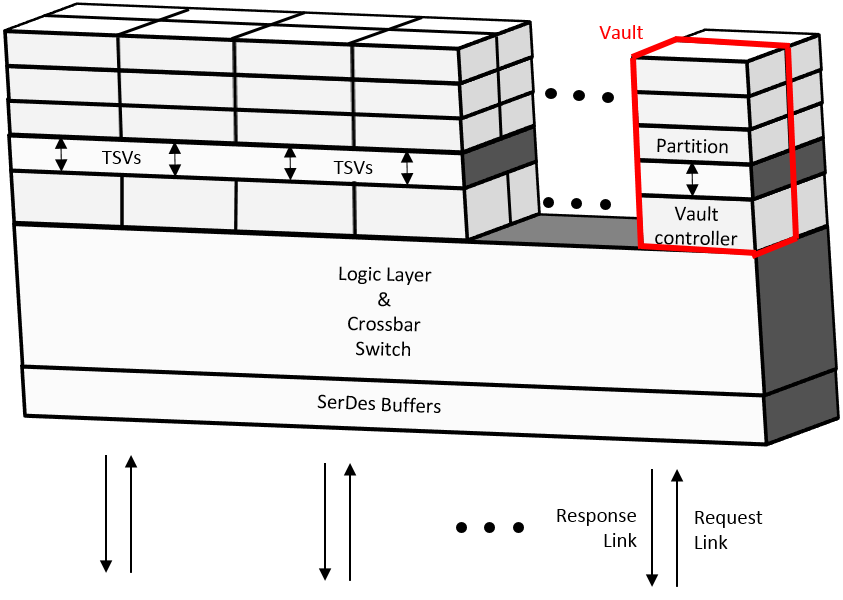
\includegraphics[width=0.75\linewidth]{figure/HMC_structures.png}
\caption{An example structure of a HMC chip }
\label{HMC-structure}
\end{figure}

TODO: Mention that HMC hosts the memory controller, and therefore direct comparisons between regular DDR DRAM and HMC is harder or less accurate. Additionally, there are "multiple" controllers, which inehrently will increase latency. What are each of them doing more specifically?

Unlike DIMMs, which are either connected with pins and fastened with plastic clips or soldered at manufacturing, the HMC is designed to be included on the same substrate as the processor, known as 2.5D integration. This shortens the host-cube data paths, which requires less power to drive compared to the relatively long buses used with DDR memory. However, as with other stacked technologies, the issue with heat generation within the stack remains and might exceed the DRAM chips' maximum operating temperature of 85 °C \cite{7459470}. This could damage the chips and render the entire stack unusable. There are a number of proposed methods to solve this, either by static or dynamic memory mappings based on thermal properties. Hsieh et al shows what different mappings could look like, where memory is spread out in such a way that heat generation is as even as possible \cite{Hsieh:2013:TMM:2501626.2512457}. Additionally, since the logic (bottom) die is used for all accesses it will produce a lot of heat either way and therefore memory mapping should be done such that as little heat as possible is produced close to another hot spot.

The underlying network enables communication between processor and memory, as well as other connected memory cubes. 
TODO: Talk more about the network itself. Crossbar switch, SerDes (and what it means), routing, pakethantering etc. The protocol (WHICH?!?!? Between what?!) used enables all cubes to address any local (?) vault, which means that one or more hosts can be placed anywhere in the network and still be able to access the entire memory. Additionally, the available support for error correction is extra important as the target market is HPC. TODO: Implications of having ECC memory; at least reference to SDRAM section where ECC is explained. 

\subsection{Interface}
Whereas DDR is designed so that the memory controller has full control over everything that happens, and the DRAM devices themselves are ''dumb'' devices, HMC moves the memory logic into the bottom cube layer and the vault controllers. In DDR communication, DRAM commands was sent directly from the CPU to the memory and got memory chunks in return. Here instead, the CPU communicates with the cube -- or a set of cubes, if that is the case -- over a general protocol, which then at the receiving end (the logic layer) is converted into the device specific protocol. Unlike with DDR, this enables manufacturers to change the internal structure of the memory without having any compatibility issues with processors. Additionally, using an abstract interface enables less memory controller complexity inside the processor, which now only have to work with load/store operations instead of handling DRAM commands. TODO: Perhaps mention that this is showing one of the advantages of having things stacked, as it does not take up any horisontal space on the CPU die to do it this way.
\bigskip

One of the main advantages of HMC is that it is made to be included on the same substrate as the processor, which shortens data paths dramatically compared to DIMMs attached to a PCB. In theory, this should lower the time it takes for data to travel to and from main memory, and also decrease the amount of energy needed to drive the buses. However, HMC also supports being soldered to the PCB, but that could potentially nullify this advantage in efficiency compared to DDRx memory. Thus, it is strongly recommended that cubes are on the same package \cite{hybrid2013hybrid}.
\bigskip

TODO: Talk about HMC's networking capabilities, how it can connect to a host and/or other cube (which is then not near memory, NUMA). Inter-processor communication via HMC net? Start creating a "problem scenario" here, where we eventually "want to know the answer". Security implications by having access to not only your memory, possibly?

\subsection{Versions of HMC}
The first announcement of HMC was made public in 2011, and the 1.0 specification was published shortly thereafter. TODO: Also a version 1.1. It uses the architecture and interface described above, and links could utilise a maximum speed of 15GB/s. In 2014, the 2.0 specification was released, and specified a doubled maximum link speed to 30GB/s \cite{hybrid2014hybrid}. There are multiple versions of HMC being tested and produced currently, with everything from 2GB to 4GB cubes and with differing speeds. Future development consists of increasing the memory size of the HMC. There are upcoming Intel processors which have been announced to use HMC 1.0 on board \cite{micron2014ikl}, but there has as of yet not been any mentions of products using 2.0. 


%%%%%%%%%%%%%%%%%%%%%%%%%%%%%%  HBM  %%%%%%%%%%%%%%%%%%%%%%%%%%%%%%
\section{High Bandwidth Memory}
High Bandwidth Memory is, unlike HMC, a standard accepted by JEDEC \cite{standard2013high}. Even though they have a few similarities, they are targeting different markets and price segments. Whereas HMC is focused on HPC applications, where money usually is less of an objection, HBM was exclusively developed for graphics hardware. It is still a stacked memory technology, and enables high bandwidth through parallelism and wide data interfaces.

\subsection{Architecture}
The stacked DRAM dies inside a HBM are accessed through \emph{channels}, where a maximum of eight channels per stack is split up between the layers. Figure \ref{HBM-structure} shows an example, with 4 DRAM dies using 2 channels per die. These channels are fully independent, using separate clocks, timings and commands. Every channel uses a 128-bit wide interface, which with a maximum of eight channels gives a 1024-bit wide interface. Furthermore, each channel can transfer data at a rate of 1-2 Gb/s. Together with the wide data interface, HBM has the potential to deliver a bandwidth of 128-256 GB/s per stack. Each channel can handle data capacities of up to 32 Gb, and with a maximum of eight channels, HBM has a maximum size of 32 GB. 
\bigskip

Figure \ref{HBM-structure} also depicts that there is an optional logic die present. This die is optional, both in its existence and in its implementation, and for example, a vendor may use it as a full memory controller. As the channels support Error-Correcting Code (ECC) memories, a controller could easily be made to support this as well. Even though the target market of HBM (graphics) might not be the most likely to need ECC, it is an available feature and could for, e.g., scientific applications be a welcome addition. 

\begin{figure}[!h]
\centering
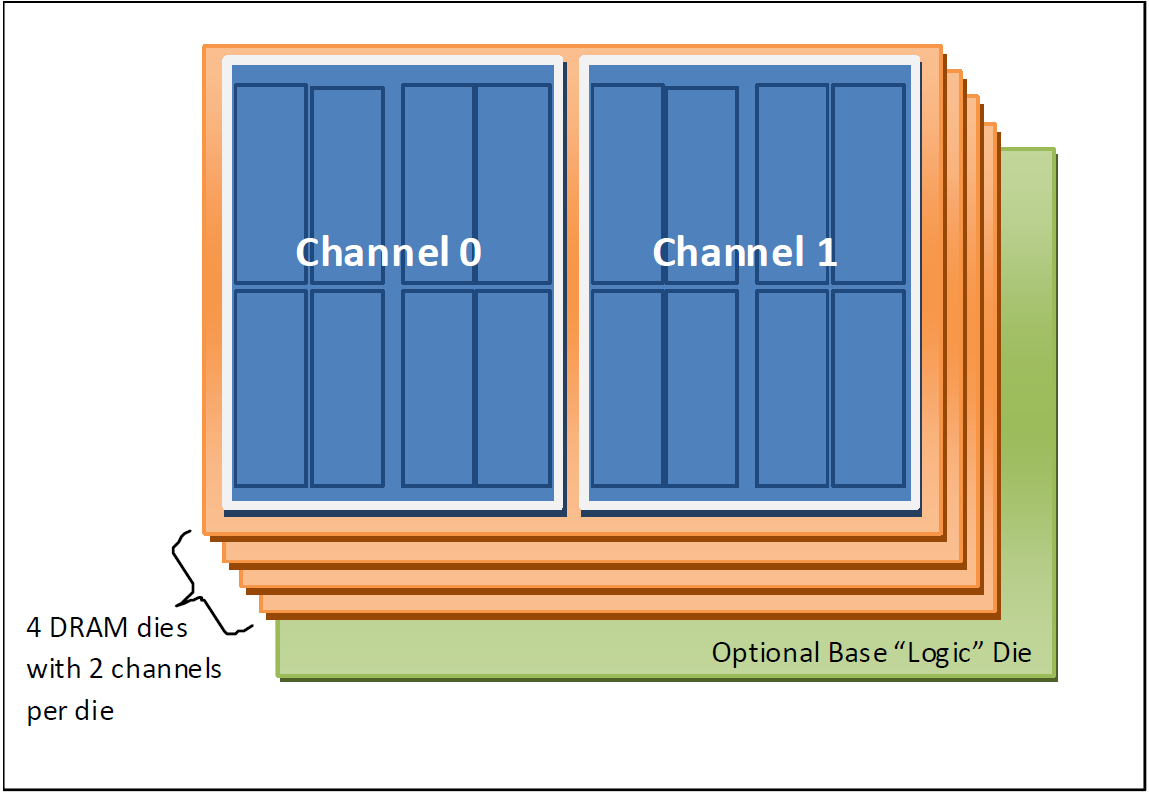
\includegraphics[width=0.75\linewidth]{figure/HBM_structure.PNG}
\caption{The structure of a HBM chip. Image courtesy of JEDEC 2013 }
\label{HBM-structure}
\end{figure}

\subsection{Interface}
The fact that there is an optional logic die included in the specification allows vendors to chose to integrate HBM with existing designs, utilising an already present memory controller, or they can choose to create a new one. The latter option may allow them to fit more components on the processor die, and make the memory part simpler. However, since the interface is different from that of DRAM, an existing memory controller would still need to be updated according to HBM specification. Even so, this provides a flexible way to more easily allow quick adoption of the memory type. TODO: Source and/or example would be great here.
\bigskip

Like with HMC, HBM is based on a 2.5D silicon interposer integration, which means that the stacked DRAM chips are placed beside the processor. In contrast to HMC, however, HBM does not support being built on the PCB. Because of its very wide interface, it would require too much energy to power those buses. Thus, HBM is required to be built close to the processor on the same substrate.

\subsection{Versions of HBM}
TODO: Find out the differences between HBM and HBM2. What has changed? 
TODO: Both HBM and HBM2 has been used in products from both AMD and Nvidia, but seems to be replaced by GDDR5X and GDDR6. There are speculations as to why, but probably not any scientific data present. Link to, e.g. Anandtech, Toms Hardware?


%%%%%%%%%%%%%%%%%%%%%%%%%%%%%%  WIO  %%%%%%%%%%%%%%%%%%%%%%%%%%%%%%
\section{Wide-IO}
While HBM and HMC aim at delivering as much performance as possible, Wide-IO (WIO) targets smaller, mobile devices with limited available power and small thermal envelope. Therefore, WIO targets high energy efficiency and low power consumption, rather than highest possible performance. Additionally, unlike HMC and HBM, WIO is designed for 3D chip-on-chip integration on System on Chips (SoCs). This enables even shorter, lower capacitance data paths compared to 2.5D as used by HMC and HBM. Like HBM, Wide-IO is a JEDEC standard, and was first accepted in 2011 \cite{standard2011wide}. 

\subsection{Architecture}
Wide-IO is based on stacked Single Data Rate (SDR) memory dies and uses a signalling system quite similar to that of standard DDR memories. Communication from the single memory controller is handled through four 128-bit wide physical channels. Additionally, there are four logical channels, which are controlled separately by the physical channels. The physical channels have access to all the data, control and clock logic to independently manage the logical channels. Each logical channels can have their own memory pages open while also having individual clock and power states. The Wide-IO stack can consist of between one to four DRAM dies -- called \emph{slices} -- and each part of the slice belonging to a physical channel is called \emph{rank}. Stacks can utilise capacities between 128MB up to 4GB. TODO: No apparent differentiation between logical and physical channels. Try to clarify! Similar to physical and virtual memory addresses? 
TODO: Power usage, link speed, bandwidth, advantages?

TODO: Find and insert a small graphic of WIO here!

\subsection{Interface}
The memory controller is very similar to a standard SDRAM controller. Since commands are similar to those in DDR, it makes the controllers resembling one another. The biggest difference being that that in the target market (mobile) there are more often than not only one or two memory channels available while there in Wide-IO are four. Furthermore, this means that the complexity of the controller might increase, and that it must be able to handle the increased load. TODO: Source!
\bigskip

Wide-IO is, unlike both HMC and HBM, primarily aimed at being 3D, chip-on-chip integrated. While the standard supports 2.5D integration, it is not recommended for optimal performance. However, as the latter integration technique gives rise to fewer problems, this will most likely be the initial approach. While there certainly are challenges in manufacturing stacked memory it is far from impossible to create working 3D chips with reasonable yields; Kim et al. managed to create a 4 die stack with an expected yield of 76\% \cite{kim20121}. TODO: Reference back to section talking about comparison between 2.5D and 3D integration performance and cost.

\subsection{Versions of WIO}
The first version was accepted by JEDEC in 2011, and a new specification for Wide-IO2 (WIO2) was accepted and released in 2014. WIO2 uses 64-bit wide channels instead, but the maximum amount of channels has increased to eight. It is still allowed to just use four channels, but there are no more logical channels available to further increase parallelism inside. TODO: not more logical channels than...? Since there no longer are channels which share control logic -- which physical and logical channels did previously -- each channel is now fully independent. The density of one chip has stayed the same (32Gb), but accepted desities now range from 4Gb instead of 1Gb. The main improvement lies in the maximum bandwidth stacks are capable of -- it has increased from 17GB/s to 68GB/s. Additionally, WIO2 no longer use SDR, but instead utilise DDR memory \cite{standard2014wide}. TODO: Clean this shit up, it is really hard to follow...
TODO: Investigate if MLM is helped by WIO using standard DDR signalling. Perhaps use it as scratchpad, like the article about HMC? 

\section{A Comparison of Emerging Technologies}
TODO: In order to conclusively get a justification of why we are exploring HMC, and not any of the others, we make a comparison and sort of a conclusion that HMC would be really interesting to investigate. This is not an obvious conclusion to make, I suppose, but talking about networks, the flexibility of having controllers elsewhere, enabling support for multi-host solutions etc. make for an interesting setup. 
TODO: Mention that hardware/os/scheduler support is needed with HMC, whereas HBM and/or WIO is more of a drop-in replacement. All possible to use as MLM though.
TODO: Repeat mention of different markets, power usage, bandwidth, price, difference in integration etc. 
TODO: Maturity can be mentioned as well, where HMC do, kind of exist in some Intel/Xilinx products, HBM and HBM2 is being used in commercial products, and WIO/2 is not used yet (probably due to earlier mentioned issues with 3D integration).